\documentclass[aspectratio=169,11pt]{beamer}
\usepackage[T1]{fontenc}
\usepackage{lmodern}
\usepackage{booktabs}
\usepackage{tikz}
\usetikzlibrary{arrows.meta,positioning,calc,fit}
\graphicspath{{figs/}}

% ---------------------------------------------------------------- look
\definecolor{ink}{HTML}{0B0B0B}
\definecolor{ink2}{HTML}{52514E}
\definecolor{accent}{HTML}{2A78D6}
\definecolor{orange}{HTML}{EB6834}
\definecolor{aqua}{HTML}{1BAF7A}
\definecolor{soft}{HTML}{F1F0EC}
\setbeamertemplate{navigation symbols}{}
\setbeamercolor{normal text}{fg=ink}
\setbeamercolor{frametitle}{fg=ink}
\setbeamercolor{title}{fg=ink}
\setbeamercolor{structure}{fg=accent}
\setbeamerfont{frametitle}{size=\Large,series=\bfseries}
\setbeamertemplate{itemize items}{\color{accent}\textbullet}
\setbeamertemplate{footline}{\hfill\textcolor{ink2}{\scriptsize\insertframenumber\,/\,\inserttotalframenumber}\hspace{1em}\vspace{0.6em}}
\newcommand{\takeaway}[1]{\par\vspace{0.4em}\noindent\colorbox{soft}{\parbox{\dimexpr\linewidth-2\fboxsep}{\small #1}}}
\newcommand{\nut}{$\nu_\tau$}

\title{Optimizing the TAMBO detector layout\\[0.2em]\large with a plan $\rightarrow$ placer $\rightarrow$ exact re-scoring loop}
\subtitle{Differential evolution, local search, and an LLM plan writer}
\author{Hamza Hanif \and Shahzaib Abbas}
\date{20 November 2026}

\begin{document}

\begin{frame}
  \titlepage
\end{frame}

% ---------------------------------------------------------------- 1
\begin{frame}{Idea}
  \begin{columns}[T]
    \begin{column}{0.64\textwidth}\footnotesize
      \begin{itemize}\setlength\itemsep{0.1em}
        \item TAMBO sees Earth-skimming \nut: the $\tau$ exits the mountain, decays in the air, and the shower crosses the valley onto detector units on the opposite slope.
        \item Where the $\sim$900 units/detectors sit decides what fraction of those showers trigger, reconstruct up-going, and pass quality cuts.
        \item \textbf{Site:} the official \texttt{volcano\_valley} simulation geometry (terrain mesh, 8.9 km$^2$ up to $35^\circ$ slope, 12.9 km$^2$ up to $50^\circ$).
        \item \textbf{Official arrays:} \texttt{official125} and \texttt{official150} are the reference layouts from the official simulations: regular triangular grids with 125 m or 150 m spacing laid over the valley slopes.
        \item \textbf{Can an agentic AI find a better layout at the same unit count?}
      \end{itemize}
    \end{column}
    \begin{column}{0.34\textwidth}
      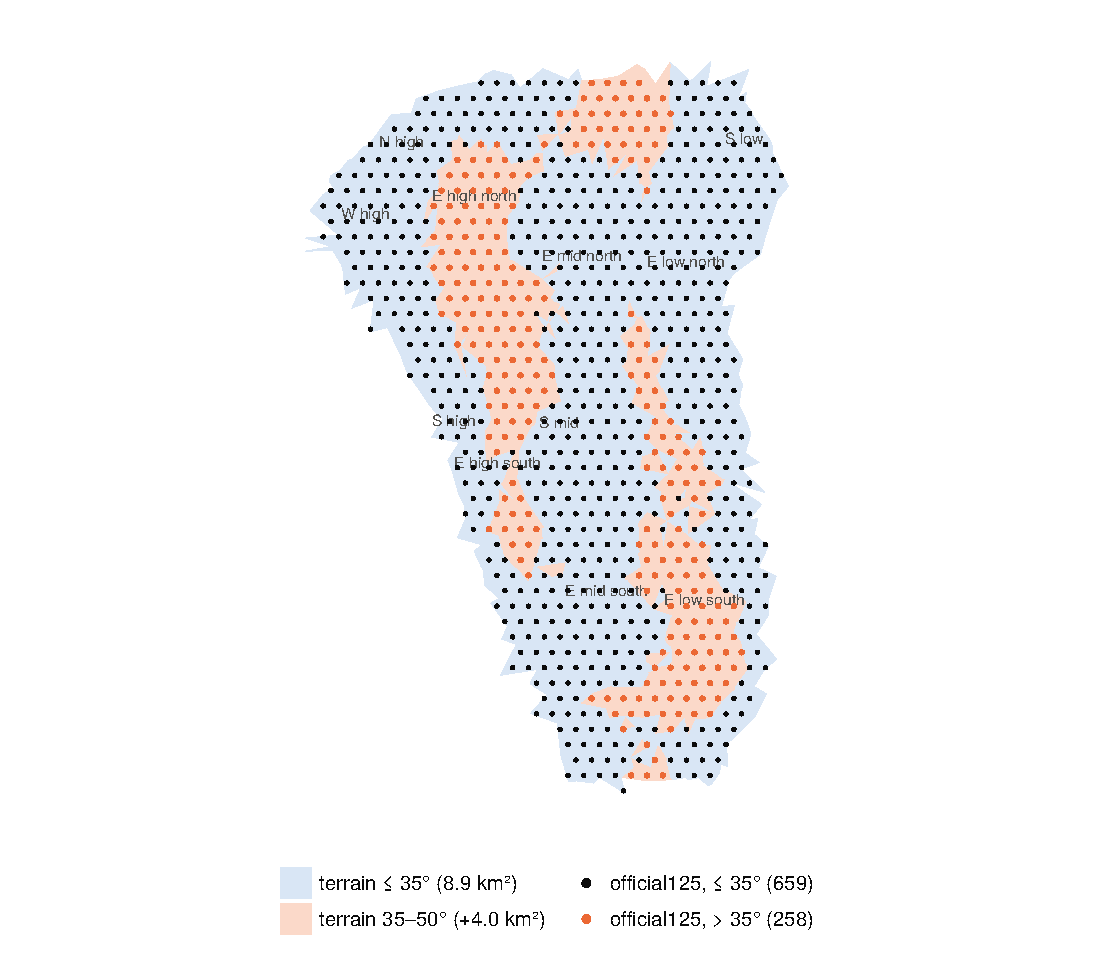
\includegraphics[width=\linewidth]{site_map.pdf}\\[-0.2em]
      {\scriptsize \texttt{volcano\_valley} terrain with the \texttt{official125} units (917).}
    \end{column}
  \end{columns}
  \vspace{0.3em}
  {\footnotesize\textbf{Constraints we set ourselves:} no new air-shower simulation (re-use the official CORSIKA surface particles); same reconstruction as the official sets (LlhamaFit, \texttt{TRIGGER\_5x1}, plane timing); a held-out event split decides, and a third (test) split stays blind until the end.}
\end{frame}

% ---------------------------------------------------------------- 2
\begin{frame}{Idea: write \emph{plans}, not coordinates (as in LLM-for-PCB-layout)}
  \centering
  \resizebox{0.97\textwidth}{!}{%
  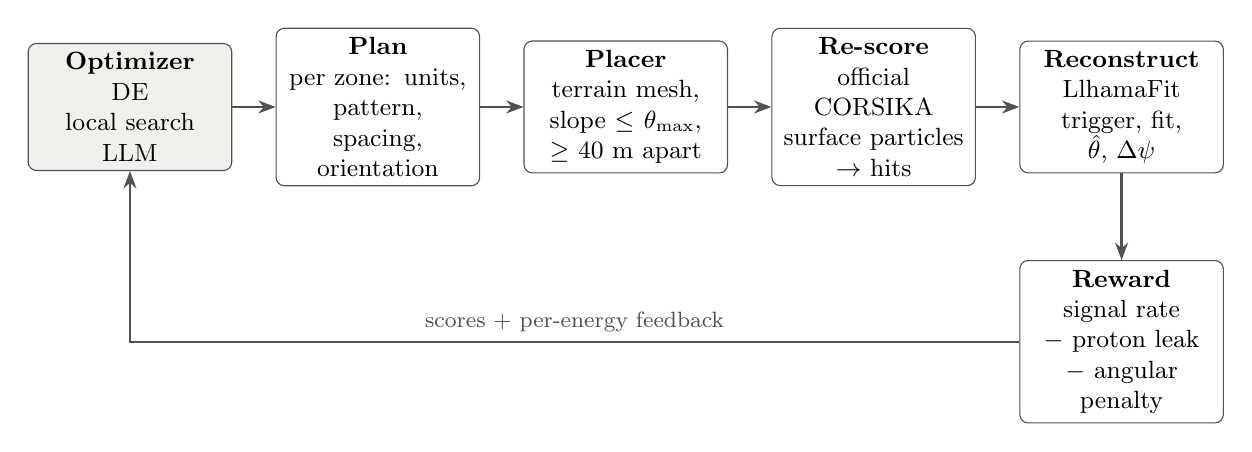
\begin{tikzpicture}[node distance=0.55cm and 0.55cm, every node/.style={font=\small},
      box/.style={draw=ink2, rounded corners=3pt, align=center, minimum height=1.25cm, text width=2.35cm, fill=white},
      opt/.style={box, fill=soft},
      arr/.style={-{Stealth[length=2.2mm]}, thick, ink2}]
    \node[opt] (opt) {\textbf{Optimizer}\\DE\\local search\\LLM};
    \node[box, right=of opt] (plan) {\textbf{Plan}\\per zone: units,\\pattern, spacing,\\orientation};
    \node[box, right=of plan] (placer) {\textbf{Placer}\\terrain mesh,\\slope $\le\theta_{\max}$,\\$\ge$ 40 m apart};
    \node[box, right=of placer] (score) {\textbf{Re-score}\\official CORSIKA\\surface particles\\$\rightarrow$ hits};
    \node[box, right=of score] (reco) {\textbf{Reconstruct}\\LlhamaFit\\trigger, fit,\\$\hat\theta$, $\Delta\psi$};
    \node[box, below=1.1cm of reco] (reward) {\textbf{Reward}\\signal rate\\$-$ proton leak\\$-$ angular penalty};
    \draw[arr] (opt) -- (plan); \draw[arr] (plan) -- (placer); \draw[arr] (placer) -- (score); \draw[arr] (score) -- (reco);
    \draw[arr] (reco) -- (reward);
    \draw[arr] (reward.west) -| node[pos=0.25, above, font=\footnotesize, text=ink2]{scores + per-energy feedback} (opt.south);
  \end{tikzpicture}}
  \vspace{0.3em}
  \begin{itemize}\scriptsize
    \item \textbf{What is a plan?} A short text recipe: for each terrain zone, how many units, in which pattern (triangular grid, contour rows, cluster, random), at what spacing and rotation. Example: ``200 units in the east-facing high zone, triangular grid, 90 m spacing''.
    \item \textbf{Role of the plan:} it is the only thing the optimizer (DE, local search, or the LLM) controls. It is small and human-readable, so it can be searched or written by an AI; the physics stays in the placer and re-scoring.
    \item The placer is deterministic: a plan always gives the same layout and score. Re-scoring is \textbf{exact} (re-mapping onto the official layout reproduces the official hits with zero mismatches).
  \end{itemize}
\end{frame}

% ---------------------------------------------------------------- 3
\begin{frame}{Objective}
  \[
    \text{reward} = 1000\, S_{\text{good}} \;-\; 10 \cdot n_{\text{proton leak}} \;-\; 2\,\max(0,\ \widetilde{\Delta\psi} - 5^\circ)
  \]
  \begin{itemize}
    \item $S_{\text{good}}$: \nut\ events / yr that trigger, are fitted, reconstruct with $\hat\theta \le 90^\circ$ and fit quality $u_3 > 0.1$ (TamboSim v1.0.1 OneWeights, reference $E^{-2.52}$ flux).
    \item Proton leak: proton showers passing the same cut (all-particle CR flux). Every good layout leaks 0.
    \item Events are split by event into \textbf{train} (optimizers see only this), \textbf{select} (choose winners), \textbf{test} (blind).
    \item Two scoring tiers: a fast tier for search (43 data parts $\times$ plan groups, single-core jobs, $\sim$10 min per 40 plans) and an exact tier for winners, with a paired event bootstrap.
  \end{itemize}
\end{frame}

% ---------------------------------------------------------------- 4


% ---------------------------------------------------------------- 5
\begin{frame}{Search methods}
  \begin{columns}[T]
    \begin{column}{0.32\textwidth}
      \textbf{\color{accent}Differential evolution}\\[0.3em]\small
      4 genes per zone (share, pattern, spacing, orientation), 11 zones. 40 plans $\times$ 20 generations. Starts from a uniform grid over all zones.
    \end{column}
    \begin{column}{0.32\textwidth}
      \textbf{\color{aqua}Local search}\\[0.3em]\small
      Moves individual units (5--40 per mutant: nudges of 20--100 m or jumps). (1+20) strategy, 30 generations, started from \texttt{official125}.
    \end{column}
    \begin{column}{0.32\textwidth}
      \textbf{\color{aqua}LLM plan writer}\\[0.3em]\small
      LLM writes 40 plans per round from the zone table, the reward, the best plans so far, and a per-energy breakdown. Same plan space, placer, and budget as DE.
    \end{column}
  \end{columns}
  \vspace{1em}
  \small Budgets: 917 units (= \texttt{official125}) and 300 units. All jobs are single-core on \texttt{serial\_requeue}; drivers resume after preemption.
\end{frame}

% ---------------------------------------------------------------- 6
\begin{frame}{DE results: allowing slopes up to 50$^\circ$}
  \begin{columns}[c]
    \begin{column}{0.5\textwidth}
      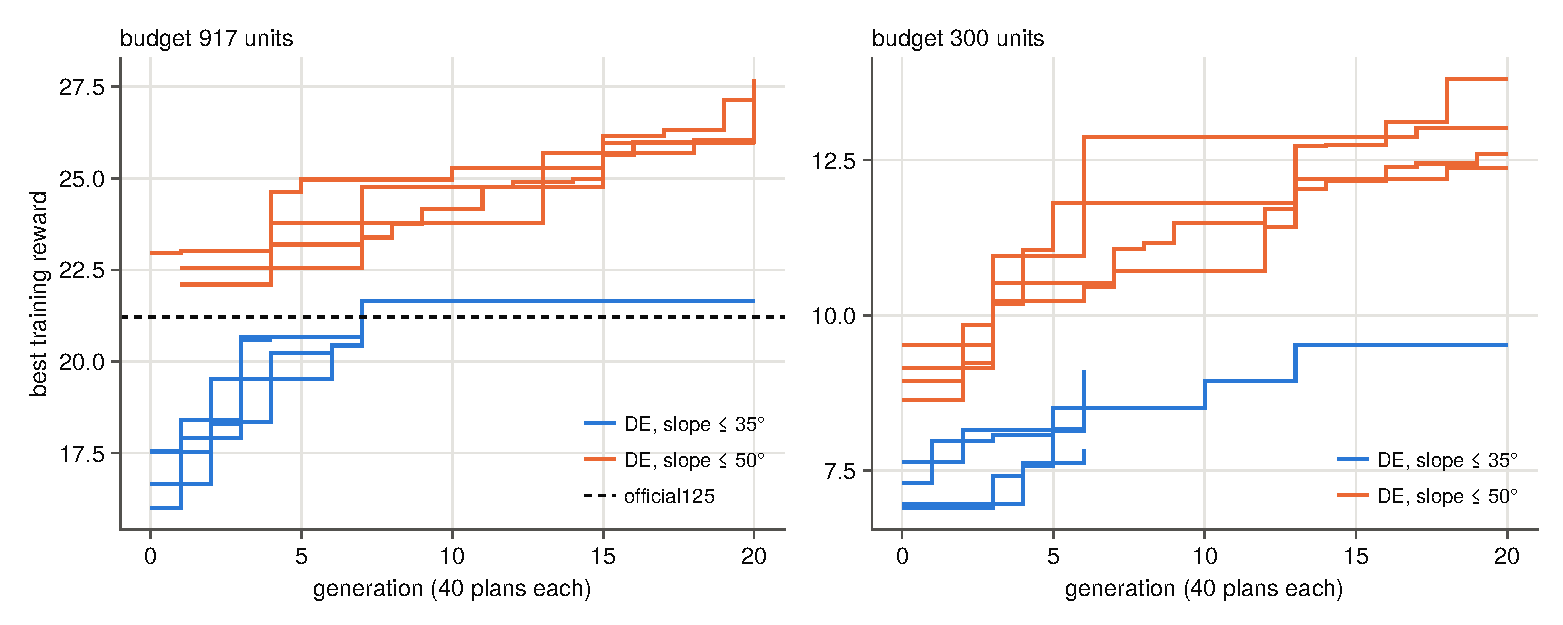
\includegraphics[width=\linewidth]{de_convergence.pdf}\\[0.2em]
      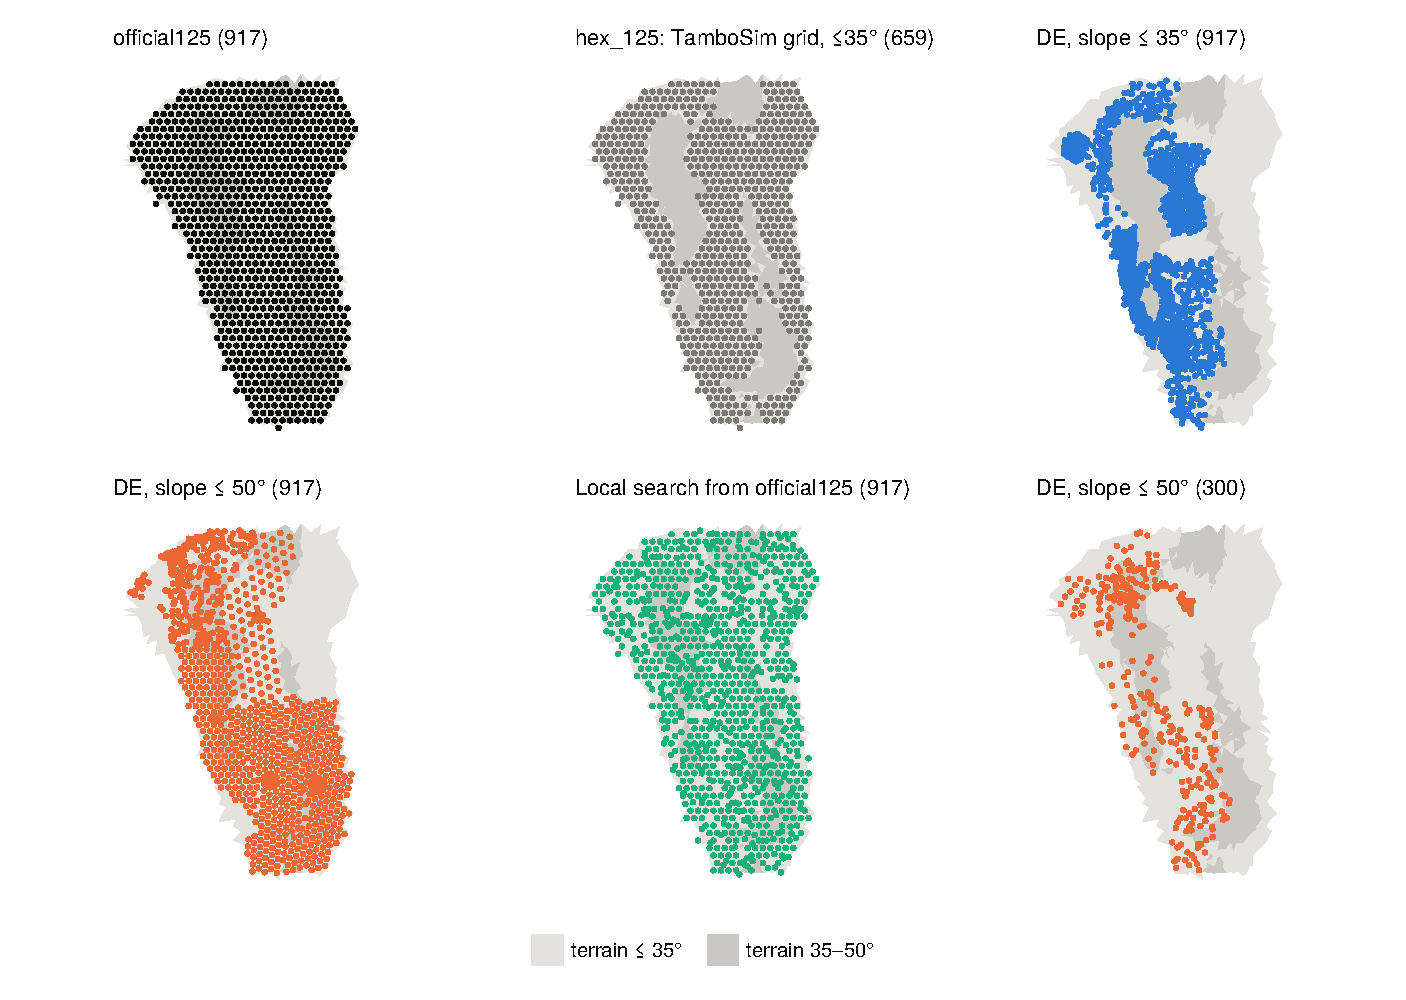
\includegraphics[width=0.85\linewidth]{layouts.pdf}
    \end{column}
    \begin{column}{0.48\textwidth}\footnotesize
      \begin{itemize}
        \item \texttt{official125} is the official 125 m grid, 917 units. 258 of them sit on 35--48$^\circ$ terrain; on terrain $\le35^\circ$ it equals TamboSim's 125 m grid.
        \item Those steep units add $\sim$70\% signal (0.0215 vs 0.0125 /yr, train).
        \item Blue: DE limited to $\le35^\circ$ ties \texttt{official125} on train and loses on held-out select (0.0199 vs 0.0256 /yr).
        \item Orange: opening terrain up to $50^\circ$ (+4.0 km$^2$) lets DE reach 26.0 vs 21.2 on train, and tie \texttt{official125} on select (0.0257 vs 0.0256 /yr, $P(\Delta>0)=0.53$).
      \end{itemize}
    \end{column}
  \end{columns}
\end{frame}

% ---------------------------------------------------------------- 7


% ---------------------------------------------------------------- 8


% ---------------------------------------------------------------- 9
\begin{frame}{Exact-tier results with a paired event bootstrap}
  \begin{columns}[c]
    \begin{column}{0.6\textwidth}
      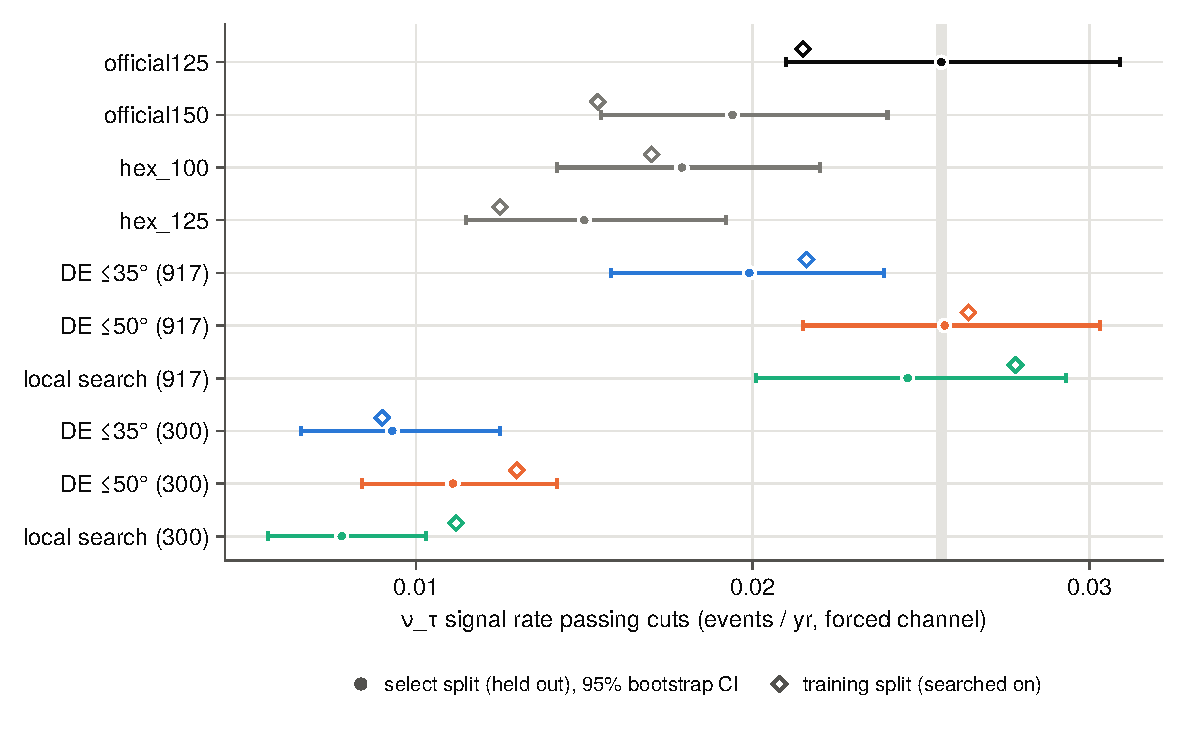
\includegraphics[width=\linewidth]{forest.pdf}
    \end{column}
    \begin{column}{0.38\textwidth}\small
      \begin{itemize}
        \item \textcolor{orange}{\textbf{DE with slopes $\le 50^\circ$}} ties \texttt{official125} on select: 0.0257 vs 0.0256 /yr, $P(\Delta>0)=0.53$. The $\le35^\circ$ DE was clearly worse ($P=0.02$).
        \item At 300 units, DE $\le 50^\circ$ beats DE $\le 35^\circ$ by $\sim$19\% on select.
        \item Select-split precision is $\sim\pm17\%$ per layout; paired differences are tighter.
      \end{itemize}
    \end{column}
  \end{columns}
\end{frame}

% ---------------------------------------------------------------- 10
\begin{frame}{Local search overfits; plan-level search generalizes}
  \begin{columns}[c]
    \begin{column}{0.44\textwidth}
      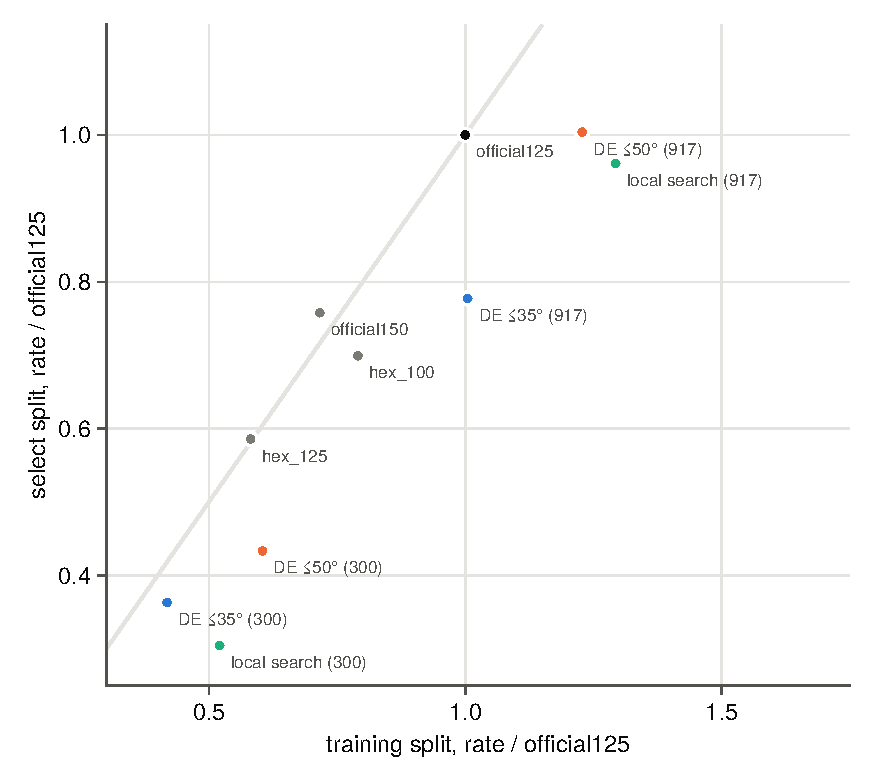
\includegraphics[width=\linewidth]{train_vs_select.pdf}
    \end{column}
    \begin{column}{0.54\textwidth}\small
      \begin{itemize}
        \item Local search moved \texttt{official125}'s units to +32\% on train (fast tier), +29\% exact, but $-4\%$ on select.
        \item Moving single units lets it catch individual training events. That is fitting noise.
        \item DE adjusts a few numbers per zone, so its train gain mostly survives on select.
        \item Every method gains on train because it picks the best of hundreds of candidates. Only the select axis counts.
      \end{itemize}
      \takeaway{Per-unit optimizers need held-out acceptance (or many more events).}
    \end{column}
  \end{columns}
\end{frame}


\begin{frame}{Benchmark layouts vs optimized layouts (917 units)}
  \begin{columns}[c]
    \begin{column}{0.56\textwidth}
      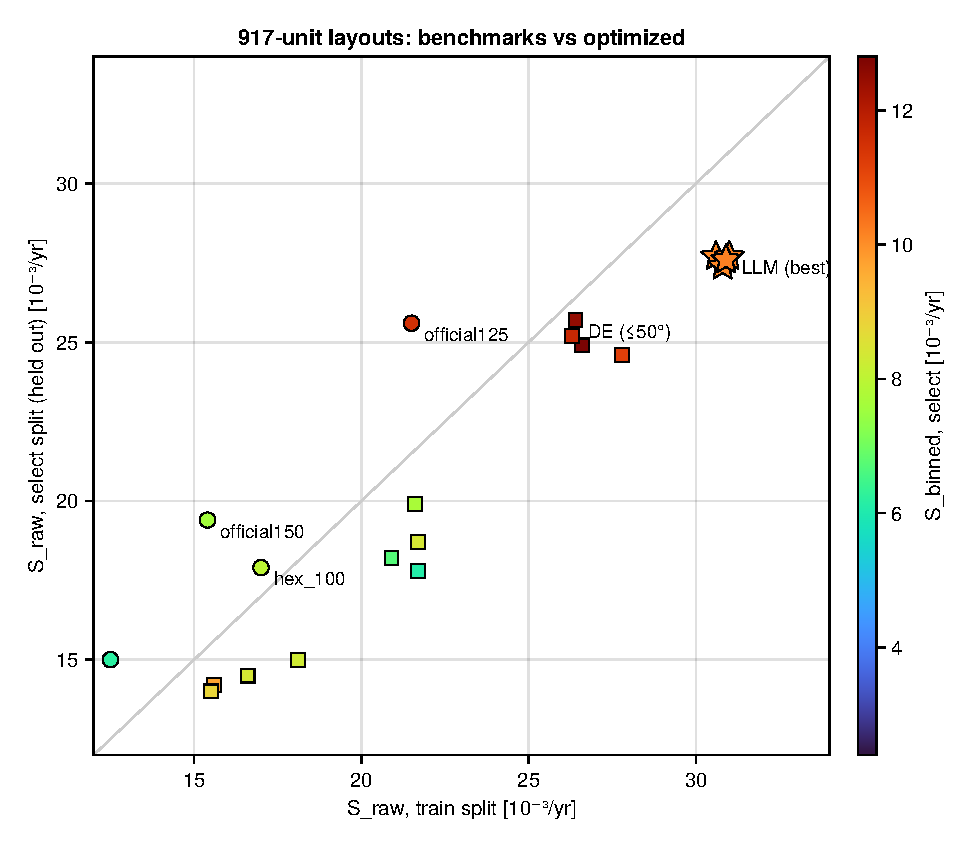
\includegraphics[width=\linewidth]{scatter_benchmarks.pdf}
    \end{column}
    \begin{column}{0.42\textwidth}\small
      \begin{itemize}
        \item Each point is one layout, scored exactly on train (x) and on held-out select events (y).
        \item Official and hex benchmarks sit lower left; the $\le\!50^\circ$ DE layouts match \texttt{official125}.
        \item The LLM layouts ($\bigstar$) are top right: ahead of \texttt{official125} on both splits.
        \item Select-split gain is $+0.0021$/yr, not yet significant ($P=0.83$).
      \end{itemize}
    \end{column}
  \end{columns}
  \takeaway{Colour: S\_binned on select, a second estimator of the same rate.}
\end{frame}


\begin{frame}{Where the units go: official125, best DE, best LLM (917 units)}
  \centering
  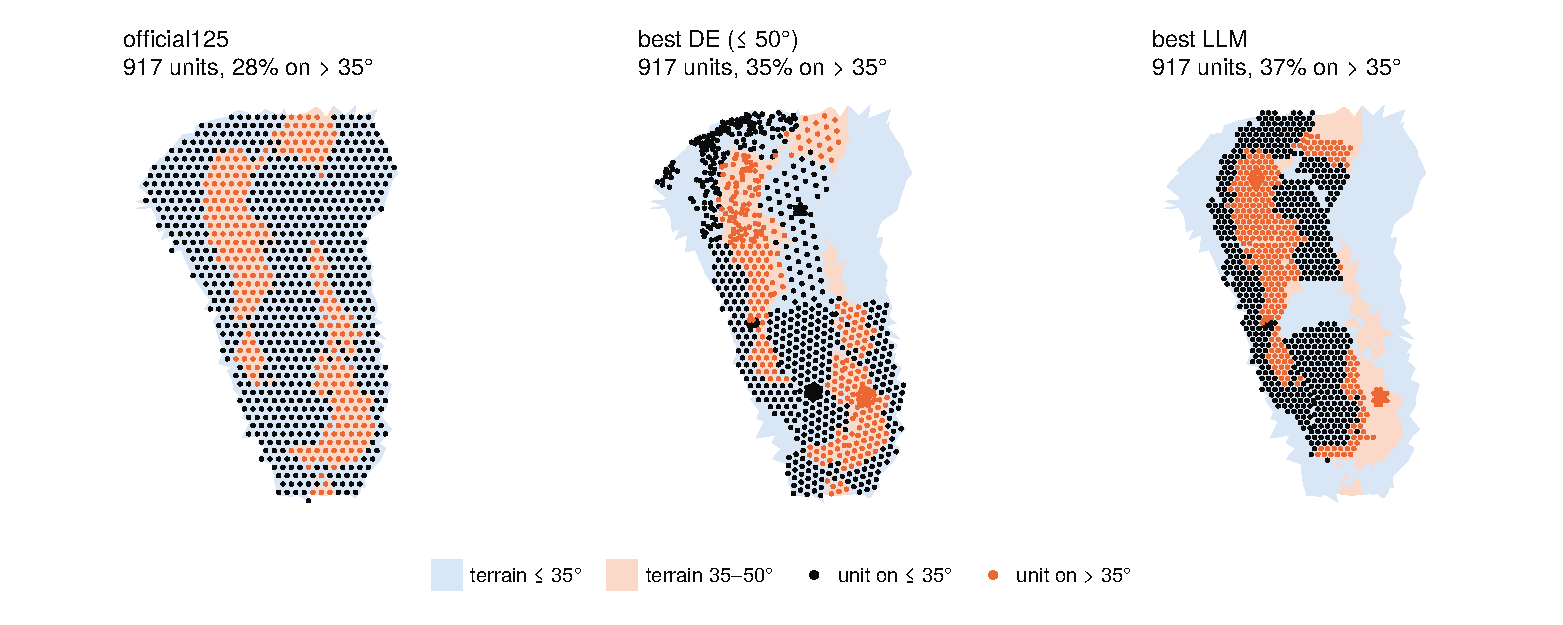
\includegraphics[width=0.97\linewidth]{terrain_three.pdf}
  \takeaway{Both optimizers move more units onto the steep (35--50$^\circ$) terrain than \texttt{official125}: 35\% (DE) and 37\% (LLM) vs 28\%.}
\end{frame}

% ---------------------------------------------------------------- 11
\begin{frame}{LLM plan writer: model and first results}
  \begin{columns}[c]
    \begin{column}{0.58\textwidth}
      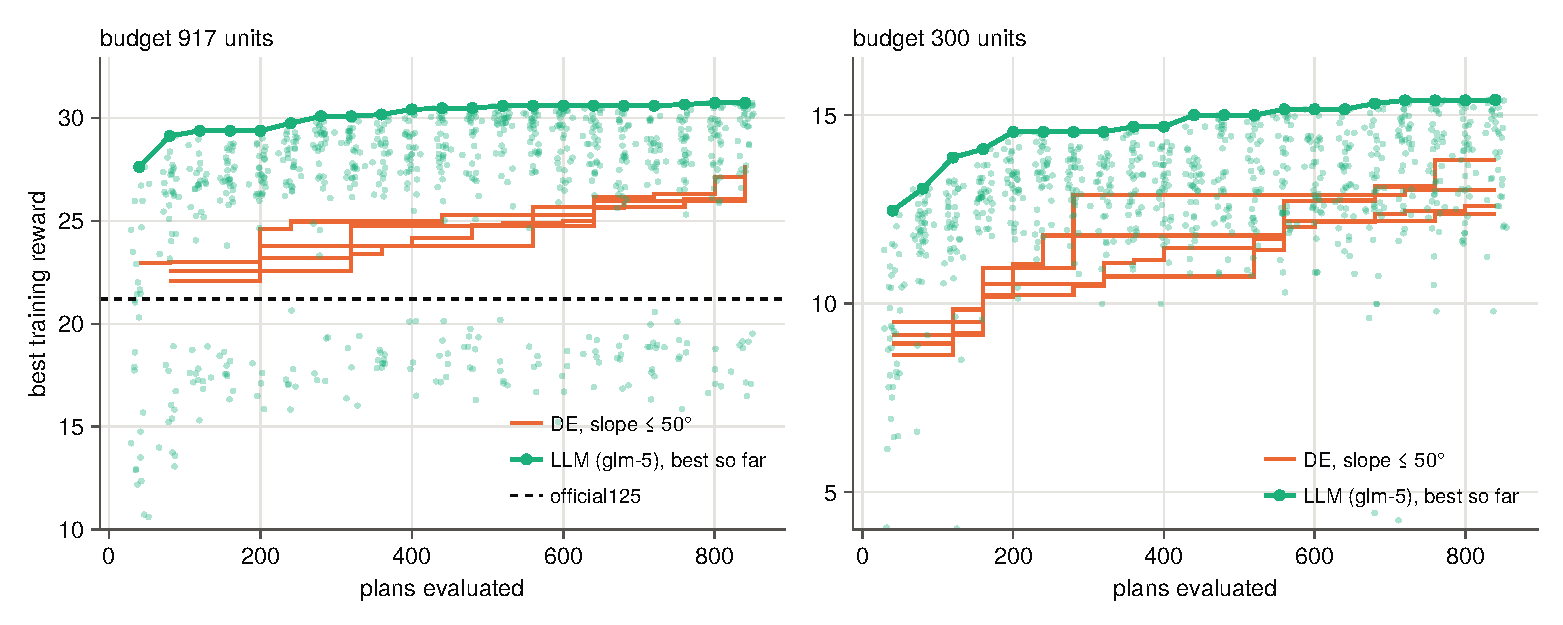
\includegraphics[width=\linewidth]{llm_vs_de.pdf}
    \end{column}
    \begin{column}{0.40\textwidth}\scriptsize
      \begin{itemize}
        \item \textbf{Model:} GLM-5, low reasoning effort; 20 rounds $\times$ 40 plans, same budget as DE.
        \item \textbf{The LLM was able to} beat both the best DE plan and \texttt{official125} on training from its very first round (27.6 at 917 units), then kept improving by refining its best plans.
        \item \textbf{Final (20 rounds, train):} 30.7 (917) and 15.4 (300), vs best DE 27.1 / 13.8 (best of 4 seeds) and \texttt{official125} 21.2.
        \item \textbf{Held-out select split:} best LLM plan 0.0277/yr vs \texttt{official125} 0.0256 ($\Delta=+0.0021$, 95\% CI $[-0.0024,+0.0066]$, $P(\Delta>0)=0.83$): promising, not yet significant. At 300 units: 0.0131 (DE 0.0111).
      \end{itemize}
    \end{column}
  \end{columns}
  \takeaway{LLM beats DE on train and is ahead of \texttt{official125} on select (P=0.83); test split still blind.}
\end{frame}

\begin{frame}{LLM plan writer: the prompt (sent for every call)}
  \small
  \begin{itemize}
    \item \textbf{System:} you design layouts for TAMBO, a $\nu_\tau$ observatory in a Peruvian valley; you write \emph{plans}, not coordinates; answer with JSON only.
    \item \textbf{Task:} write 10 new plans with exactly $N$ detector units (round $r$ of 20).
    \item \textbf{Site:} zone table (area, mean slope, elevation, centroid, capacity at 40 m spacing).
    \item \textbf{Plan format:} per zone \texttt{name, n, pattern, spacing\_m, orient\_deg} (+ \texttt{row\_step\_m}, \texttt{radius\_m}); what each pattern does; $\sum n = N$.
    \item \textbf{Objective:} reward $=1000\,S_{\rm good}-10\,n_{\rm leak}-2\max(0,\widetilde{\Delta\psi}-5^\circ)$ with definitions.
    \item \textbf{History:} the 12 best plans so far (reward, $S$, leaks, $\Delta\psi$, placed units, full plan), per-energy-set breakdown of the last round's top 3, last-round summary and weakest plans.
    \item \textbf{Instruction (varies per call):} refine the best / explore / single-change edits / combine ideas; think briefly about the physics, then output the JSON.
  \end{itemize}
\end{frame}

% ---------------------------------------------------------------- 12
\begin{frame}{Open questions for the collaboration}
  \begin{enumerate}
    \item \textbf{Deployable slope limit.} Is 35--50$^\circ$ terrain buildable? \texttt{official125} already uses 258 such units, and every result above depends on the answer.
    \item \textbf{Upstream \nut\ channel.} Is $1/\text{(surface pdf)}$, with no survival or conversion factor, the intended OneWeight? Could we get an enriched production at 0.1--10 PeV?
    \item \textbf{Proton statistics.} Good layouts leak 0--2 MC protons, so the background gate is set by counting noise. More proton and Fe showers at high energy would help.
    \item \textbf{Conventions.} Is $+x$ east? Is the TamboMakie flux the benchmark? Are $\bar\nu_\tau$ included?
  \end{enumerate}
\end{frame}

% ---------------------------------------------------------------- 13
\begin{frame}{Summary and next steps}
  \small
  \begin{itemize}
    \item A plan $\rightarrow$ placer $\rightarrow$ exact re-scoring loop works on the existing simulations, with no new CORSIKA runs.
    \item The largest single lever found so far is \textbf{terrain slope}, not pattern: the 35--50$^\circ$ band adds $\sim$70\% signal.
    \item With that band open, DE matches \texttt{official125} on held-out events. Nothing beats it significantly yet.
    \item Per-unit local search overfits. Plan-level search generalizes.
  \end{itemize}
  \vspace{0.3em}
  \textbf{Next}
  \begin{itemize}
    \item More LLM seeds/models to tighten the select-split interval; then one final test-split check.
    \item Local search with held-out acceptance.
    \item One final, unblinded evaluation on the test split.
  \end{itemize}
\end{frame}

\end{document}
